% --- IMPORTS ---
\documentclass[leqno]{article}
\usepackage{graphicx}
\usepackage{dsfont}
\usepackage{mathtools}
\usepackage{amssymb}
\usepackage{amsmath}
\usepackage{amsthm}
\usepackage{float}
\usepackage{ragged2e}
\usepackage{tensor}
\usepackage{fancyhdr}
\usepackage{empheq}
\usepackage[most]{tcolorbox}
\usepackage{enumitem}
\usepackage{dirtytalk}
\usepackage{marginnote}
\usepackage{microtype}
\usepackage[
  a4paper,
  left=0.8in,
  right=1in,
  top=1in,
  bottom=0.5in,
  headheight=14pt,
  headsep=0.4in
]{geometry}
\setlength{\parindent}{0cm}
% --- TikZ Packages ---
\usepackage{pgfplots}
\pgfplotsset{compat=1.18}
\usepgfplotslibrary{fillbetween, polar}
\usetikzlibrary{calc, positioning}
\usetikzlibrary{angles, quotes}
\usetikzlibrary{arrows.meta}
\usetikzlibrary{decorations.pathreplacing, decorations.markings}
\usetikzlibrary{patterns}
\usetikzlibrary{intersections}
% --- URL Packages ---
\usepackage[colorlinks=true,linkcolor=red,citecolor=magenta,urlcolor=black]{hyperref}%
\urlstyle{same}
% --- END OF IMPORTS ---

% --- CUSTOM COMMANDS ---
\RenewDocumentCommand{\marks}{o m}{%
  \IfValueTF{#1}%
    {\marginnote{\raggedright\textbf{[#2]}}[#1]}%
    {\marginnote{\raggedright\textbf{[#2]}}}%
}
\newcommand{\vspacerule}[2]{%
  \par\vspace*{#1}%
  \noindent\hrulefill\par
  \vspace*{#2}%
}
\definecolor{scarlet}{RGB}{205, 40, 75}
\newcommand{\questionitem}{%
  \item\phantomsection
  \addcontentsline{toc}{section}{Question \number\value{enumi}}%
}
\renewcommand{\contentsname}{Questions}
% --- END OF CUSTOM COMMANDS ---

% --- HEADER CONFIG ---
\pagestyle{fancy}
\fancyhead{}
\fancyfoot{}
\renewcommand{\headrulewidth}{0.9pt}
\lhead{De Moivre's Theorem}
\chead{}
\rhead{\href{https://danieljsmith.org}{danieljsmith.org}}
% --- END OF HEADER CONFIG ---

\begin{document}
\vspace*{20pt}
\tableofcontents
\newpage
\begin{enumerate}[
  label=\textbf{\arabic*.},
  leftmargin=*,
  topsep=0pt,
  partopsep=0pt,
  parsep=0pt
]

% ---- Question 1 ----
\questionitem

A complex number $z$ has modulus $1$ and argument $\theta$. \\
\begin{enumerate}[label=\textbf{(\alph*)}]
  \item Show that
  \[
  z^n + \frac{1}{z^n} = 2\cos n\theta
  \quad\text{and}\quad
  z^n - \frac{1}{z^n} = 2\mathrm{i}\sin n\theta,
  \qquad n \in \mathbb{Z}^+
  \]
  \marks[-20pt]{3}
  \item Hence, by expanding $\left(z + \frac{1}{z}\right)^3$ and $\left(z - \frac{1}{z}\right)^3$, show that
  \[
  \tan 3\theta = \frac{3\tan\theta - \tan^3\theta}{1 - 3\tan^2\theta}
  \]
  \marks[-20pt]{4}
\end{enumerate}

\newpage

% ---- Question 2 ----
\questionitem

\begin{enumerate}[label=\textbf{(\alph*)}]
  \item Using de Moivre's theorem, show that
  \[
  \sin^4\theta\cos^2\theta \equiv \frac{1}{32}(\cos 6\theta - 2\cos 4\theta - \cos 2\theta + 2)
  \]
  \marks[-20pt]{5}
  \item By using the substitution $\alpha=\left(\frac{\pi}{2}-\theta\right)$, or otherwise, find a similar identity for $\sin^2\theta\cos^4\theta$. \marks{3} \\
  \item Given that $0<a<\frac{\pi}{2}$ and
  \[
  \int_0^a \left(\sin^4\theta\cos^2\theta + 2\sin^2\theta\cos^4\theta\right)\,\mathrm{d}\theta = \frac{\pi}{32} - \frac{\sqrt{3}}{64}
  \]
  find the exact value of $a$. \marks{5} \\
\end{enumerate}

\newpage

% ---- Question 3 ----
\questionitem

Use de Moivre's theorem to find the constants $A$, $B$ and $C$ in the identity
\[
\sin\theta\cos^4\theta = A\sin\theta + B\sin 3\theta + C\sin 5\theta
\]
\marks[-20pt]{4}


\newpage

% ---- Question 4 ----
\questionitem

\begin{enumerate}[label=\textbf{(\roman*)}]
  \item Starting with the result
  \[
  e^{\mathrm{i}\theta}=\cos\theta+\mathrm{i}\sin\theta
  \]
  show that
  \begin{enumerate}[label=(\Alph*)]
    \item
    \[
    \left(\cos\theta+\mathrm{i}\sin\theta\right)^n=\cos n\theta+\mathrm{i}\sin n\theta
    \]
    \marks[-20pt]{2}
    \item
    \[
    \sin\theta=\frac{1}{2\mathrm{i}}\left(e^{\mathrm{i}\theta}-e^{-\mathrm{i}\theta}\right)
    \]
    \marks[-20pt]{2}
  \end{enumerate}
  \item Using the result in part (i)(A), obtain the values of the constants $a$, $b$, $c$, $d$ and $e$ in the identity
  \[
  \cos 8\theta \equiv a\sin^8\theta+b\sin^6\theta+c\sin^4\theta+d\sin^2\theta+e
  \]
  \marks[-20pt]{6}
  \item Using the result in part (i)(B), obtain the values of the constants $P$, $Q$, $R$, $S$ and $T$ in the identity
  \[
  \sin^8\theta \equiv P\cos 8\theta+Q\cos 6\theta+R\cos 4\theta+S\cos 2\theta+T
  \]
  \marks[-20pt]{6}
  \item Hence show that
  \[
  \sin \frac{\pi}{8}=\left(\frac{17-12\sqrt{2}}{64}\right)^{\frac{1}{8}}
  \]
  \marks[-20pt]{3}
\end{enumerate}

\newpage


% ---- Question 5 ----
\questionitem

\begin{enumerate}[label=\textbf{(\alph*)}]
  \item Use de Moivre's theorem to show that $\cos 6\theta \equiv (1 - 2\sin^2\theta)(16\sin^4\theta - 16\sin^2\theta + 1)$ \marks{5} \\
  \item By solving the equation $\cos 6\theta = 0$, deduce that $\sin^2\left(\frac{\pi}{12}\right) = \frac{2 - \sqrt{3}}{4}$. \marks{4} \\
  \item Hence, or otherwise, write down the exact values of $\sin^2\left(\frac{5\pi}{12}\right)$, $\sin^2\left(\frac{7\pi}{12}\right)$ and $\sin^2\left(\frac{11\pi}{12}\right)$. \marks{3} \\
\end{enumerate}

\newpage

% ---- Question 6 ----
\questionitem

Let $t=\tan\theta$. By writing
\[
\cos\theta+\mathrm{i}\sin\theta=\cos\theta\,(1+\mathrm{i}t)
\]
and expanding $(1+\mathrm{i}t)^6$, use de Moivre's theorem to show that
\[
\tan 6\theta=\frac{6\tan\theta-20\tan^3\theta+6\tan^5\theta}{1-15\tan^2\theta+15\tan^4\theta-\tan^6\theta}
\]
\marks[-30pt]{7}

\newpage


% ---- Question 7 ----
\questionitem

\begin{enumerate}[label=\textbf{(\alph*)}]
  \item Use de Moivre's theorem to show that
  \[
  \sin 6x = \sin 2x\left(a\cos^4 x + b\cos^2 x + c\right)
  \]
  where $a$, $b$ and $c$ are integers to be determined. \marks{4} \\
  \item Hence solve, for $0<\theta<\frac{\pi}{2}$,
  \[
  \sin 6\theta = \sin 2\theta \cos 2\theta
  \]
  giving your answers to $3$ decimal places. \marks{4} \\
\end{enumerate}

\newpage

% ---- Question 8 ----
\questionitem

\begin{enumerate}[label=\textbf{(\alph*)}]
  \item By considering the binomial expansion of $(z-z^{-1})^6$, where $z=\cos\theta+\mathrm{i}\sin\theta$, use de Moivre's theorem to show that
  \[
  \sin^6\theta=\frac{1}{32}\bigl(10-15\cos 2\theta+6\cos 4\theta-\cos 6\theta\bigr)
  \]
  \marks[-20pt]{5}
  \item Hence, using the substitution $x=\tan\theta$, find the exact value of
  \[
  \int_0^1 \frac{x^6}{(1+x^2)^4}\,\mathrm{d}x
  \]
  \marks[-30pt]{4}
\end{enumerate}

\newpage

% ---- Question 9 ----
\questionitem

\begin{enumerate}[label=\textbf{(\alph*)}]
  \item Use de Moivre's theorem to show that
  \[
  2\cos 5\theta = 32\cos^5\theta - 40\cos^3\theta + 10\cos\theta
  \]
  \marks[-20pt]{4}
  \item Hence solve the equation
  \[
  x^5 - 5x^3 + 5x + 1 = 0
  \]
  giving all roots in the form $2\cos q\pi$, where $q$ is a rational number. \marks{4} \\
\end{enumerate}

\newpage


% ---- Question 10 ----
\questionitem

\begin{enumerate}[label=\textbf{(\alph*)}]
  \item If $n$ is a positive integer and $z = \cos\theta + \mathrm{i}\sin\theta$, show that
  \[
  z^n + \frac{1}{z^n} = 2\cos n\theta,
  \qquad
  z^n - \frac{1}{z^n} = 2\mathrm{i}\sin n\theta
  \]
  \marks[-20pt]{2}
  \item By considering $\left(z+\frac{1}{z}\right)^3\left(z-\frac{1}{z}\right)^2$, find constants $A$, $B$ and $C$ such that
  \[
  \sin^2\theta\cos^3\theta = A\cos 5\theta + B\cos 3\theta + C\cos\theta
  \]
  \marks[-20pt]{6}
\end{enumerate}

\newpage

% ---- Question 11 ----
\questionitem

\begin{enumerate}[label=\textbf{(\alph*)}]
  \item By writing $1+\mathrm{i}\tan\theta = \sec\theta(\cos\theta + \mathrm{i}\sin\theta)$ and using de Moivre's theorem, show that
  \[
  (1+\mathrm{i}\tan\theta)^4 = \frac{\cos 4\theta + \mathrm{i}\sin 4\theta}{\cos^4\theta}
  \]
  \marks[-20pt]{3}
  \item Expand $(1+\mathrm{i}\tan\theta)^4$ and hence show that
  \[
  \cos 4\theta = \frac{1-6\tan^2\theta+\tan^4\theta}{(1+\tan^2\theta)^2}
  \]
  and
  \[
  \sin 4\theta = \frac{4\tan\theta(1-\tan^2\theta)}{(1+\tan^2\theta)^2}
  \]
  \marks{4} \\
  \item Deduce that
  \[
  \tan 4\theta = \frac{4\tan\theta(1-\tan^2\theta)}{1-6\tan^2\theta+\tan^4\theta}
  \]
  \marks[-20pt]{2}
\end{enumerate}

\newpage

% ---- Question 12 ----
\questionitem

\begin{enumerate}[label=\textbf{(\alph*)}]
  \item Use de Moivre's theorem to show that
  \[
  \sec 6\theta = \frac{\sec^6 \theta}{32 - 48\sec^2 \theta + 18\sec^4 \theta - \sec^6 \theta}
  \]
  \marks[-30pt]{6}
  \item Hence obtain the roots of the equation
  \[
  x^6 - 18x^4 + 48x^2 - 32 = 0
  \]
  in the form $\sec(q\pi)$, where $q$ is rational. \marks{4} \\
\end{enumerate}

\newpage

% ---- Question 13 ----
\questionitem

\begin{enumerate}[label=\textbf{(\alph*)}]
  \item Use de Moivre's theorem to show that
  \[
  \cos 5\theta = 16\cos^5 \theta - 20\cos^3 \theta + 5\cos \theta
  \]
  \marks[-20pt]{5}
  \item Hence solve for $0 \le \theta \le \pi$
  \[
  16\cos^5 \theta - 20\cos^3 \theta + 5\cos \theta = \cos 2\theta
  \]
  giving your answers as exact multiples of $\pi$. \marks{5} \\
\end{enumerate}

\newpage

% ---- Question 14 ----
\questionitem


\begin{enumerate}[label=\textbf{(\alph*)}]
  \item Use de Moivre's theorem to determine constants $A$, $B$ and $C$ such that
  \[
  \cos^5 \theta \equiv A\cos 5\theta + B\cos 3\theta + C\cos \theta
  \]
  \marks[-20pt]{5}
\end{enumerate}


\begin{figure}[H]
    \centering
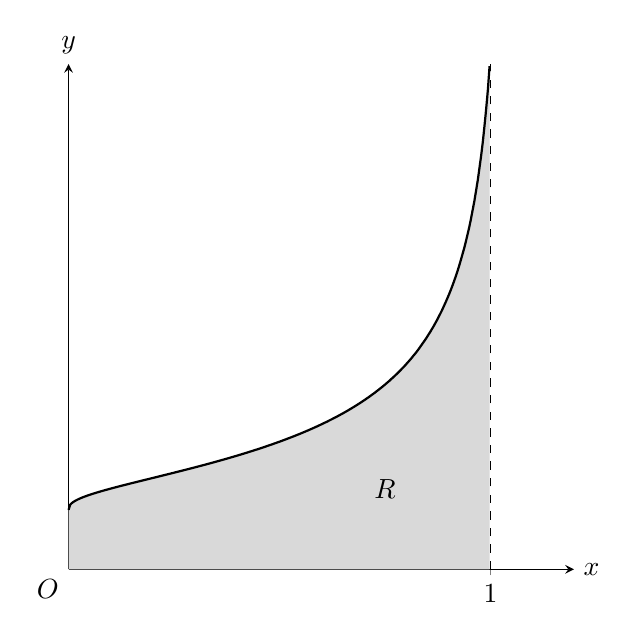
\begin{tikzpicture}
\begin{axis}[
    axis lines=left,
    xlabel={$x$},
    ylabel={$y$},
    xmin=0, xmax=1.15,
    ymin=0, ymax=8.5,
    xtick={0.96},
    xticklabels={$1$},
    ytick=\empty,
    width=8cm,
    height=8cm,
    clip=false,
    every axis x label/.style={at={(ticklabel* cs:1)}, anchor=west},
    every axis y label/.style={at={(ticklabel* cs:1)}, anchor=south}
]
\addplot[draw=none, fill=gray!30, domain=0:0.958, samples=250] {1/sqrt(1 - pow(x,1/3))} \closedcycle;
\addplot[thick, black, domain=0:0.958, samples=250] {1/sqrt(1 - pow(x,1/3))};
\addplot[dashed, black] coordinates {(0.96,0) (0.96,8.5)};
\node[below left] at (axis cs:0,0) {$O$};
\node at (axis cs:0.72,1.35) {$R$};
\end{axis}
\end{tikzpicture}
\end{figure}


The function $f$ is defined by
\[
f(x)=-3\sin\left(5\cos^{-1}\left(x^{\frac{1}{6}}\right)\right)-25\sin\left(3\cos^{-1}\left(x^{\frac{1}{6}}\right)\right)-150\sin\left(\cos^{-1}\left(x^{\frac{1}{6}}\right)\right), \qquad 0\le x<1
\] \\
\begin{enumerate}[label=\textbf{(\alph*)}, resume]
  \item Show that
  \[
  f'(x)=\frac{40}{\sqrt{1-x^{\frac{1}{3}}}}
  \]
  \marks[-20pt]{6}
\end{enumerate}
The diagram shows the curve with equation
\[
y=\frac{1}{\sqrt{1-x^{\frac{1}{3}}}}
\] \\
for $0\le x<1$ and the asymptote $x=1$. The region $R$ is the unbounded region between the curve, the $x$-axis, the line $x=0$ and the line $x=1$. \\
You are given that the area of $R$ is finite. \\
\begin{enumerate}[label=\textbf{(\alph*)}, resume]
  \item Determine the exact area of $R$. \marks{3} \\
\end{enumerate}

\newpage

% ---- Question 15 ----
\questionitem

\begin{enumerate}[label=\textbf{(\roman*)}]
  \item Use de Moivre's theorem to show that
  \[
  \cos 5\theta \equiv \cos \theta \left(1 - 12\sin^2 \theta + 16\sin^4 \theta\right)
  \]
  \marks[-20pt]{5}
  \item Hence determine the range of values of
  \[
  \frac{\cos 5\theta}{\cos \theta}
  \]
  given that $\cos \theta \ne 0$. \marks{7} \\
\end{enumerate}

\newpage


% ---- Question 16 ----
\questionitem

\begin{enumerate}[label=\textbf{(\alph*)}]
  \item Use de Moivre's theorem to show that
  \[
  \cos 5\theta = 16\cos^5 \theta - 20\cos^3 \theta + 5\cos \theta
  \]
  \marks[-20pt]{5}
  \item Use the identity given in part (a) to find the $2$ positive roots of
  \[
  64x^5 - 80x^3 + 20x + 1 = 0
  \]
  giving your answers to $3$ significant figures. \marks{4} \\
\end{enumerate}

\newpage

% ---- Question 17 ----
\questionitem

\begin{enumerate}[label=\textbf{(\alph*)}]
  \item Use de Moivre’s theorem to show that
  \[
  \sin^2 \theta \cos^2 \theta = \frac{1}{8}(1-\cos 4\theta)
  \]
  \marks[-20pt]{5}
  \item Hence, or otherwise, find the solution of the differential equation
  \[
  \frac{\mathrm{d}y}{\mathrm{d}\theta} - 2y\tan \theta = \sin^2 \theta
  \]
  for which $y=0$ when $\theta=\frac{1}{4}\pi$. \marks{6} \\
\end{enumerate}

\newpage

% ---- Question 18 ----
\questionitem

\begin{enumerate}[label=\textbf{(\alph*)}]
  \item Use de Moivre’s theorem to show that
  \[
  \cos^6 \theta = a \cos 6\theta + b \cos 4\theta + c \cos 2\theta + d
  \]
  where $a$, $b$, $c$ and $d$ are constants to be found. \marks{5} \\
  \item Hence show that
  \[
  \int_0^{\pi/4} \cos^6 \theta \, \mathrm{d}\theta = \frac{11}{48} + \frac{5\pi}{64}
  \]
  \marks[-30pt]{5}
\end{enumerate}
\end{enumerate}
\end{document}
